\chapter{Attacks}

In the previous chapter, we saw two basic attacks: the Fan-Out and the Nakamoto Race.
The Fan-Out is more of a misconfigured network situation, because no mining adversary
is required to mount it. The Nakamoto Race is a foundational attack.
It will function as a prototype for other attacks which we will explore in this chapter.

In this chapter, we will talk about how the various ledger virtues we defined in the
last chapter can be broken by adversaries of varying mining power. Because ledger virtues
follow from chain virtues, the adversary will have to break the chain virtues first.
So we will look at \emph{examples} of attacks that break the chain virtues. Remember,
if we describe an attack that works, this is sufficient to illustrate that the system
is broken. However, if an attack we think about happens \emph{not} to work, this is not
sufficient to argue that the system is secure. We may have just happened to think of
the wrong attack.

\section{Attacks of a Minor Adversary}\index{Minor Adversary}

A minor adversary is an adversary for which $t < n - t$. This is also known as
a $< 50\%$ attack. What virtues can such an adversary break? Let us go over all the
virtues in question and explore how much an adversary can break them.

\subsection*{Common Prefix}
As we saw in the last chapter, it is possible to have \emph{good} or
\emph{bad} configurations of the system if the parameters $T$ and $k$ are set incorrectly
when the $\Delta$, $t$, $n$, $q$ that exist on the network are taken into account.
For example, consider the extreme value
$T = 2^\kappa$. Then every query is a successful query, and every successful query
failed to be a convergence opportunity. Then, if there are multiple honest parties
$n - t > 1$, it doesn't make a difference how much we wait for $k$; we will never
have convergence. As such, Common Prefix is not achieved, and therefore safety is
violated. In these very misconfigured networks, the adversary can cause a Common
Prefix violation even with no mining power, just by allowing the honest parties
to diverge on their own.

However, in proper blockchain protocol configurations, the density of convergence
opportunities will be more than the density of adversarially successful queries.
In these cases, \emph{the best attack that a minor adversary can do is to perform the
Nakamoto Attack}~\cite{nakamoto-wins}. As we've seen, using this attack she cannot break Common Prefix,
except with negligible probability in $k$. The more we allow $k$ to grow, the more the actual successful
queries of the adversary and the actual convergence opportunities will tend to
approximate their expectations. We will make this argument precise when we
prove the Common Prefix against \emph{all} adversaries in Chapter~\ref{chapter:earnest3}.

\subsection*{Chain Growth}
Even though a minor adversary can affect the chain velocity $\tau$ of honest
parties by stopping her mining, she cannot prevent the rest of the honest network
from mining. If she is a minority adversary, this can mean she can drop the expected
chain growth rate to at worse $\frac{1}{2}$ of what it would be were she to mine honestly.
\emph{The best strategy for harming chain growth is simply not to mine}.
Even if the adversary mines withheld chains in the fashion that the Nakamoto Race
attack does, these chains will not be adopted, unless they are longer than what
the honest parties have adopted. In these cases, even though the honest parties are
switching from one chain to another, the chain they are switching to is still longer
than what they have, and so Chain Growth is happening.

\subsection*{Chain Quality}
For a minor adversary to harm Chain Quality, she would have to try and supress as many
honestly generated blocks as possible from becoming adopted by honest parties. Ideally,
she wants honest parties to adopt chains that only consist of adversarially generated blocks.

In case the adversary plays honestly, and no forks occur on the chain, then the number of
blocks she gets is proportional to her mining power. The honest adversary\footnote{The
\emph{honest adversary} is not a misnomer. Remember that the adversary controls any party which
we did not designate as honest. She can do whatever she wishes with that party -- including
playing honestly.}
therefore achieves quality $\mu = \frac{n - t}{n}$. This matches our expectation that
the proportion of blocks on a chain generated by a particular party match his mining power.

\section{Selfish Mining}
We might try to think about different strategies in which the adversary may
try to harm quality. There is an adversarial strategy known as \emph{Selfish Mining}\index{Selfish Mining}
which is a modified version of the Nakamoto Race, and specifically targets the minimization
of the quality of the honestly adopted chain.

The adversary works as follows. Initially, all honest parties start at some block $B$.
Similar to the Nakamoto Race, the honest parties and the adversary mine on separate forks,
both extending $B$. If at any point of time the adversary finds a block on her fork, she keeps
it secret, similarly to the Nakamoto Race. She can keep growing her secret fork more and more.
If at any point in time the honest parties find a block, then the adversary wishes to suppress
it from the honestly adopted chain. There are two cases: Either she has at least one withheld
block up her sleeve on her secret fork, or she does not. If, when the honest parties mine a block,
the adversary does not have a withheld block up her sleeve, then there isn't much she can do.
Since she doesn't have any secret blocks, she accepts that the honestly mined block that was
just broadcast will be accepted as part of the honestly adopted chain, and restarts mining
her secret fork on top of the honestly generated block.

On the contrary, if
she has one or more withheld blocks up her sleeve, she releases exactly \emph{one} of her
withheld blocks in an attempt
to kick out the block produced by the honest party from the honestly adopted chain. If
the adversary's block makes it to the doorstep of other honest parties before the honestly
mined block arrives, the adversarially generated block will be adopted, and the
honestly generated block will be rejected.
The adversary keeps the rest of her withheld blocks secret so that they can be used in the
future.

Whether the adversarial block can make it to the doorstep of an honest party before the
honest block makes it there is an issue of how well positioned the adversary is on the
network. Remembering our threat model, we want to make the adversary as powerful as possible,
so that, when the time comes to prove the security of our protocol, the proof of security
will be the strongest. As such, we will assume that the adversary has significantly better
network presence than the honest parties. We model this as follows. Whenever any honest party
broadcasts a message to the network, the adversary gets a chance to see it \emph{first},
prior to any other honest party seeing it. The adversary then has the choice to broadcast
her own message \emph{prior} to the honest message making its way. In this way, the adversary
can \emph{rush ahead} in her message delivery as compared to the honest message delivery.
She can \emph{frontrun} honest messages after seeing them so that adversarial messages
get delivered prior to the honest message. We call such an adversary a
\emph{Rushing Adversary}\index{Rushing Adversary}. This may seem like giving too much power
to the adversary, but is not an unreasonable assumption in practice. When we deploy our real
systems, we want to give assurances to honest parties even if they have very basic network
connectivity, for example through a slow Internet connection in a remote area. On the contrary,
it is rather inexpensive for the adversary to buy good network presence by deploying some
servers on central Internet backbone locations. This would allow the adversary to actually
mount rushing attacks against parties located on the Internet's last mile quite successfully.

% TODO: algorithm for the selfish miner

The basic idea of the selfish ming attack is that, whenever the adversary has a headstart of secretly
kept blocks, any honest mining power goes to waste, because any blocks produced by the honest
parties during those moments will be kicked out by the competing blocks broadcast by the rushing
adversary.

This is a more complicated attack than what we've seen before, so let's look at an example
execution of the attack. The example is illustrated in Figure~\ref{fig.selfish-mining}. The
honestly generated blocks are colored blue, while the adversarially generated blocks are
colored red. The final honestly adopted chain is displayed at the bottom and consists of a
mixture of honestly generated and adversarially generated blocks, whereas abandoned honest
blocks are seen at the top as temporary forks. The blocks are numbered in the order they were
mined. As you can see, adversarially mined blocks are never abandoned. The only blocks ever
abandoned are honestly mined. Additionally, all temporary forks have a length of exactly $1$.
The example begins with everyone having genesis. Initially, both the adversary and the honest
parties attempt to mine a block on top of genesis. An honest party manages to get a block first,
and this is block $1$. As the adversary does not hold any withheld blocks, she adopts block
$1$, and so does every other honest party. Now the honest parties and the adversary all mine
on top of block $1$. At this point, the adversary manages to get block $2$, but keeps it secret.
Now the adversary is mining on top of block $2$, but the honest parties are mining on top of
block $1$. At this point, the adversary gets lucky and manages to mine another block $3$
on top of block $2$. She keeps both block $2$ and block $3$ secret. Now the adversary is mining
on top of block $3$, but the honest parties are still mining on top of block $1$. An honest
party manages to get block $4$ and broadcasts it to the network. The adversary
sees this block being broadcast on the network and rushes to send her own block $2$ in order to
suppress honest block $4$. Since the adversary is rushing, she manages to get block $2$ on
the doorstep of every honest party prior to them seeng block $4$. Therefore every honest
party (beyond the one who mined block $4$) now adopts block $2$ and keeps mining on top of it.
Note how the honest mining power that went into mining block $4$ went completely to waste
here, because the adversary knew ahead of time that she would be able to replace this block.
Now every honest party is mining on top of block $2$, but the adversary is still ahead and
mining on top of block $3$. The honest parties generate block $5$, but the adversary counters
by releasing block $3$. The adversary maintains her lead by finding $6$, and rushes it out upon
seeing $7$. At this point, both the honest parties and the adversary have adopted and are mining
on top of block $6$, and the adversary has no headstart any more.

The honest parties manage to get block $8$, which the adversary is forced to accept, since she
has no withheld blocks at this time. Next, she gets $9$ and keeps it secret. The honest parties
get $10$, but the adversary uses $9$ to suppress it. At this point, both the honest parties
and the adversary are mining on $9$. The adversary gets $11$. The honest parties get $12$ and
the adversary suppresses it with $11$. The honest parties get $13$, which the adversary accepts.
Next, the adversary gets $14$. The honest parties get $15$, and the adversary suppresses it with
$14$. Lastly, the honest parties get $16$ and everybody adopts it.

\begin{figure}[h]
    \centering
    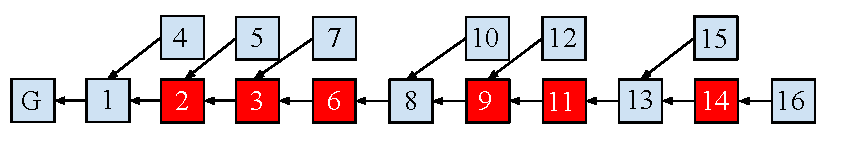
\includegraphics[width=\columnwidth,keepaspectratio]{figures/selfish-mining.pdf}
    \caption{The selfish mining attack in action. Red blocks (2, 3, 6, 9, 12, 14) are adversarially
             generated, whereas blue blocks are honestly generated.}
    \label{fig.selfish-mining}
\end{figure}

We wish to discover how low the chain quality $\mu$ gets for various values of
$\frac{t}{n}$. This attack seems harder to analyze analytically, so we will use a simulation
method to analyze its effectiveness. In the simulation, we will code a simplified model of the attack
in which the honest parties only get convergence opportunities, and there are no successful queries
that are not convergence opportunities. This gives an advantage
to the honest parties, so, if our adversary is successful against these honest
parties, she is definitely going to also be successful against more modest honest parties
who also have to deal with the lack of convergence opportunities. We use this simplification
because we consider temporary forks due to network desynchronization immaterial to the attack in
question, and we want to get an approximate feeling for how the chain quality behaves.

The pseudocode for the simulation is illustrated in Algorithm~\ref{alg.selfish-simulation}.
This simulation uses the Monte Carlo\index{Monte Carlo} method: An experiment is repeated many times
(Line~\ref{alg.selfish-simulation.monte-carlo}),
and a quantity of interest (here, the chain quality $\mu$) is measured during each experiment
(Line~\ref{alg.selfish-simulation.mu}). An average
is then taken across all experiment executions
(Line~\ref{alg.selfish-simulation.avg}). The hope is that, even though each experiment may
yield an unusual value, the average value will be indicative of the attack's nature.

Each experiment proceeds as follows.
Initially, all honest parties have
only the genesis block, so all honestly adopted chains have just one honest
block (Line~\ref{alg.selfish-simulation.genesis}). Each experiment allows the chain
adopted by the honest parties to grow until it reaches a predetermined length $c$
(Line~\ref{alg.selfish-simulation.chain}). While blocks are produced in the experiment,
the simulation keeps track of how many blocks adopted by the honest parties have
been honestly generated (\textsf{honest}), as well as how many blocks adopted by the honest parties
have been adversarially generated (\textsf{adversary}). The simulation also keeps track
of the number of blocks the adversary has generated but is still keeping secret (\textsf{advantage}).
At every iteration, we allow one block to be mined, and we give the block to
the adversary with probability $\frac{t}{n}$, or to the honest parties with
probability $\frac{n - t}{n}$. This is done by selecting a uniformly random
number in the interval $[0, 1)$ and then comparing it with $\frac{t}{n}$ (Line~\ref{alg.selfish-simulation.random}).
For simplicity, as discussed before, we assume
all honestly generated blocks are instantly communicated to the rest of the honest
parties, so no divergence occurs between honest parties. Nevertheless, the rushing adversary
has the option to rush whenever an honest block has been produced, and the adversary has
an advantage.

If the honest parties get a block, then the adversarial advantage is checked.
If the adversary has no advantage, this means that the number of honestly generated
blocks in the honestly generated chain increases by one (Line~\ref{alg.selfish-simulation.honest}),
and the adversary starts
mining on top of the new honestly generated block. The adversarial advantage remains $0$.
If the adversary has a positive advantage, then the adversary broadcasts one of the previously
secret blocks, and so displaces the honestly generated block, which is discarded by
all honest parties. In this simple simulation, we ignore the fact that the honest party
who mined this block will keep mining on it. This is an accurate simplification if the
mining parties are many, with a small amount of mining power each. This causes the
adversarially generated block to become honestly adopted, and the adversarial advantage
to decrease by one (Line~\ref{alg.selfish-simulation.adv}). Lastly, if the adversary
happens to get a new block, then this block is kept secret for the moment, and the
adversarial advantage increases by one (Line~\ref{alg.selfish-simulation.withhold}).

The Monte Carlo method is a very useful method to get an initial feel of whether
an attack can be successful and to analyze probabilities and other values of interest.
While it is not an analytical method, it can often function as a first indicator
of whether an attack makes sense, and whether further theoretical analysis is warranted.
It can also be used as a mechanism to double-check our theoretical results.

\import{./}{algorithms/alg.selfish-simulation}

Plugging some numbers into this simulation, we observe that, for large values of $c$
and $m$, the average chain quality converges to $\frac{1}{2}$ for $\frac{t}{n} = \frac{1}{3}$,
and to $0$ as $\frac{t}{n} \rightarrow \frac{1}{2}$. You are asked to verify these
results in Problem~\ref{problem:selfish-simulation}.

We used a simulation to calculate these numbers to get a feel for them, but we can also
support these numbers theoretically and to develop a closed-form formula for the achieved
chain quality. To see how this attack performs, note that \emph{every} adversarially
mined block is accepted in the honestly adopted chain. For every adversarially generated
block that is accepted on the honest chain, there is one honestly generated block that
was displaced from the honestly adopted chain. Those are exactly the honestly generated
blocks that are wasted. The rest of the honestly generated blocks make it to the honestly
adopted chain.

Let $L$ be the total number of blocks produced, of which $L_\mathcal{A}$ are
adversarial and $L_h$ are honest. The ratio $\frac{L_\mathcal{A}}{L}$ will
approach $\frac{t}{n}$, the ratio $\frac{L_h}{L}$ will approach
$\frac{n - t}{n}$, and the ratio $\frac{L_\mathcal{A}}{L_h}$
will approach $\frac{t}{n - t}$ after long executions.
Let $|\chain|$ denote the length of the
ultimate honestly adopted chain, $|\chain_\mathcal{A}|$ be the number of
adversarial blocks in it, and $|\chain_h|$ be the number of honest blocks
in it. We have that $|\chain_\mathcal{A}| = L_\mathcal{A}$ since all
honestly generated blocks are eventually adopted, but
$|\chain_h| = L_h - L_\mathcal{A}$, since every adversarially generated
block displaces an honest block. Lastly,
$|\chain| = |\chain_\mathcal{A}| + |\chain_h| = L_h$.
The overall chain quality will be
$\mu = \frac{|\chain_h|}{|\chain|} = \frac{L_h - L_\mathcal{A}}{L_h} = 1 - \frac{t}{n - t} = \frac{n - 2t}{n - t}$.
This verifes our simulation results.

The conclusion is that a minor adversary with close to $50\%$ mining power can bring
chain quality very close to $0$. Regardless, if the adversary has mining power strictly
less than $50\%$, the chain quality will be non-zero.
Incidentally, the fact that in the above calculations
$|\chain| = L_h$ also shows that the selfish mining attack is minimizing \emph{both}
chain quality \emph{and} chain growth at the same time, since the adversarially mined
blocks do not contribute to the honestly adopted chain growing more than it would
grow even if no adversarial blocks were to be mined.

A minor adversary cannot break Common Prefix for large $k$, can reduce but not eliminate the chain velocity
$\tau$, and can reduce Chain Quality to $\mu$ close to, but not equal to $0$, the minor adversary cannot
break the ledger virtues. Safety survives because of Common Prefix. Liveness survives because the chain grows
and the chain quality is non-zero. Remember that, to ensure liveness, it is required that just a single honest
block survives once in a while. While the time it takes for transactions to confirm will be harmed, all honest
transactions will eventually make it to the ledger of all honest parties, and these ledgers will remain
consistent.

\section{Attacks of a Major Adversary}\index{Major Adversary}
We have explored the attacks of a minor adversary, and showed that ledger virtues survive them in a
well-configured blockchain network. Let us now turn our attention to a \emph{major adversary}, an
adversary with $t > n - t$. Such attacks are also known as $51\%$ attacks (or $> 50\%$ attacks).

\subsection*{Common Prefix}
A major adversary can easily break Common Prefix by performing the Nakamoto Race, as discussed
in the previous chapter. In fact, the larger the duration of the race, the more blocks the adversary
gets. Increasing the Common Prefix $k$ parameter in our confirmation rule does not help!
Concretely,
if the honest parties have converged to a tip $B$, the adversary can start mining on top of
$B[{:}{-1}]$. Once she has mined $k + 2$ blocks and holds a chain $\chain_\mathcal{A}$,
she waits for the honest parties to also mine their own $k$ blocks on top of $B$
forming the chain $\chain$.
She then releases her chain and, since it is longer, the honest parties switch to it.
The Common Prefix property is violated because, prior to the switch, the honest parties
were holding a chain whose stable chunk $\chain[{:}{-k}]$ was not a prefix of the
adversarially produced unstable chain $\chain_\mathcal{A}$. In particular,
$\chain[{:}{-k}][-1]$ does not appear in $\chain_\mathcal{A}$. Refer back to
Figure~\ref{fig.nakamoto-race}
for a visualization.

\subsection*{Chain Quality}
A major adversary can easily break Chain Quality and achieve exactly $\mu = 0$ by, again,
performing the Nakamoto Race. In fact, the adversary can simply just ignore all honest blocks,
and mine on her own from the genesis block. No matter what the honest parties do, she will eventually
surpass them and build a longer chain. The honest parties will adopt the adversarially generated
chain. Since the adversarially generated chain only consists of adversarially generated blocks
(with the exception of the genesis block), the chain quality of the chain chunk $\chain[1{:}]$
will be $0$.

\subsection*{Chain Growth}
For the same reasons that a minor adversary fails to completely eliminate Chain Growth, the
major adversary also fails to eliminate Chain Growth. The best attack the adversary can perform
is to remain idle. Then velocity $\tau$ then drops to roughly a proportion $\frac{n - t}{n}$ of the rate
it would have if the adversary were honest. Nevertheless, if $n - t > 0$, the chain continues
to grow. The fact that the adversary cannot significanty harm Chain Growth is a consequence of
the longest chain rule of our protocol.

\subsection*{Safety}
Since the major adversary can break Common Prefix, she can also break ledger safety. The double
spending attack using the Nakamoto Race is one example. A transaction that is rolled back from
an honest party's ledger and then replaced by a different transaction in the same position
is a safety violation.

As we discussed when we first introduced the double spending attack in Chapter~\ref{chapter:transaction},
the double spending is problematic because it has real-world ramifications. When the adversary double
spends, she receives some real-world goods, such as a car. When a conflicting transaction appears on
the ledger of the seller and the original transaction is reverted, the adversary has long since
departed with her brand new car. However, note that, while the adversary can break safety, the
ledgers adopted by the honest parties are always \emph{locally consistent}. There is never the
case of an honest party adopting a ledger that contains two conflicting transactions. The only
thing that happens is that an honest party switches from one, locally consistent, ledger to another,
also locally consistent, ledger.

It is worth noting that a major adversary cannot steal an honest party's money from the system.
Spending an honest party's money would require creating a signature that validates with the honest
party's public key. That would require stealing the honest party's secret key, or breaking
the existential unforgeability property of signature schemes. Therefore, even a major adversary
cannot take our money.

A major adversary also cannot create more money than what is allowed by the macroeconomic policy,
because blocks that violate the macroeconomic policy are not accepted by the honest nodes.
Recall that when a block is validated, the coinbase transaction is checked, and part of that
check includes validating the macroeconomic policy. Even though the honest nodes are a minority,
they do not accept an invalid chain which violates these basic rules.

\subsection*{Liveness}
While the major adversary cannot break Chain Growth, she can break Chain Quality and therefore
she can cause a liveness violation. This can be used to mount censorship attacks. As soon as
the censoring adversary sees an honest transaction she dislikes, she starts mining on top of
the currently adopted block, excluding the transaction in question from her block. She
keeps mining on top of that block, eventually creating a longer chain than the honest parties
because she holds the majority of compute. She must continue to mine, because she cannot allow
any honest block to ever make it into the chain, as honest parties are still including the
transaction in question in their mempool. Contrary to a Nakamoto Race, she does not need to keep
her fork secret, and she can allow it to be extended by the honest parties at any time.

Such a situation is depicted in Figure~\ref{fig.censorship-attack}. The white circle represents
a transation that the adversary wishes to censor. Whereas the honest parties are continuously
attempting to include it into their blocks, the adversary keeps displacing their blocks by
mining on top of the parent block. The honest blocks with the transaction in question never
makes it into the ultimate honestly adopted longest chain.

\begin{figure}[h]
  \centering
  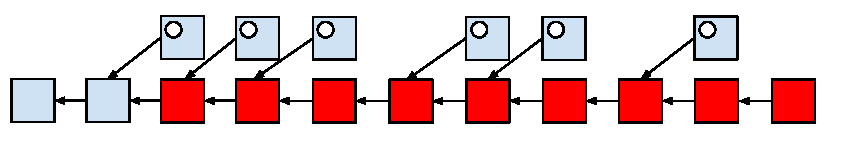
\includegraphics[width=\columnwidth,keepaspectratio]{figures/censorship-attack.pdf}
  \caption{A major adversary mounts a censorship attack.}
  \label{fig.censorship-attack}
\end{figure}

\section{Healing}\index{Healing}

Even though a major adversary can break Common Prefix, Chain Quality, Safety, and Liveness,
it is worth considering whether a these properties \emph{heal} when the adversarial power
goes back to a low value. The idea is that we may have a \emph{temporary dishonest majority},
which overtakes the network for a short duration of time, but the adversary soon goes back
to controlling the minority of compute. While we will not prove the exact formulae which
determine the healing parameters of the chain in this book, we want to give intuitive
arguments about why a proof-of-work chain heals very naturally.

The temporary dishonest majority situation is depicted in Figure~\ref{fig.temporary-dishonest}.
The system begins with a minor adversary whose compute increases until it exceeds
$50\%$. The dishonest majority compute remains for a period of time, until the adversary's
compute drops back to below $50\%$.

% TODO: redo this graph
\begin{figure}[h]
  \centering
  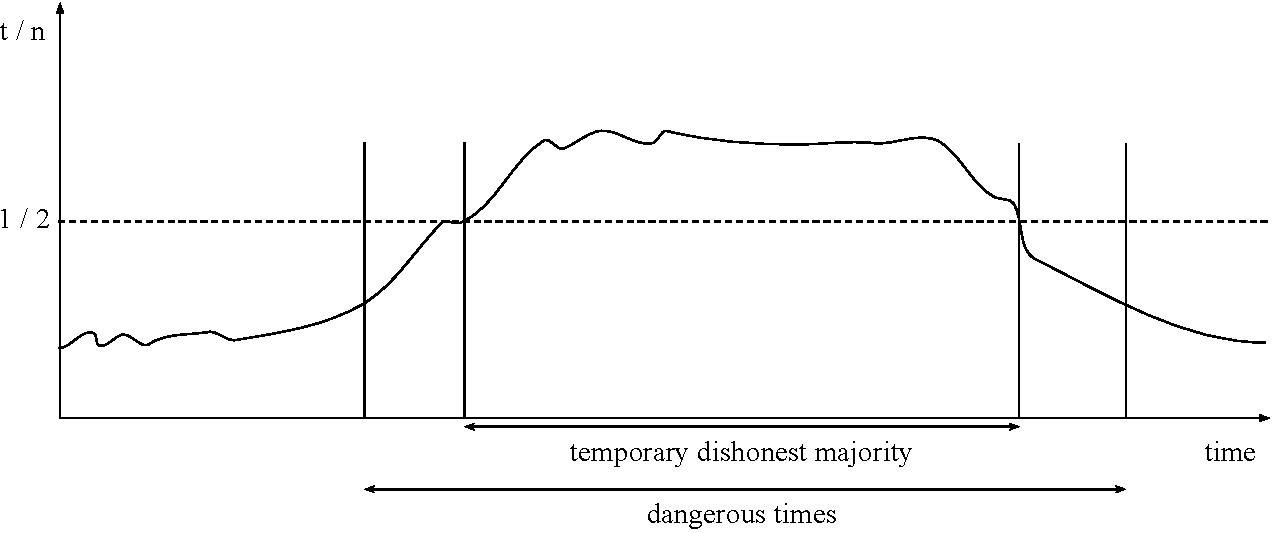
\includegraphics[width=\columnwidth,keepaspectratio]{figures/temporary-dishonest.pdf}
  \caption{The temporary dishonest majority.}
  \label{fig.temporary-dishonest}
\end{figure}

\subsection*{Common Prefix}
We already know that the major adversary can break Common Prefix, no matter what parameter
$k$ we choose. However, if she only has \emph{temporary} dishonest majority, she cannot
revive very old temporary forks, because it would take a long time to have them catch up
with the current times, so she must mine on a recent temporary fork. She will likely be
able to create a temporary fork longer than $k$ blocks long, but not \emph{arbitrarily}
longer, because she has limited time. The length of temporary forks will still be bounded.
When the adversary's mining power drops below the majority, she has limited time until
she can reveal any secret temporary forks she has mined, because the honest parties will
soon create a longer chain and the, now minor, adversary will not be able to catch up.
Hence, such withheld temporary forks will soon be useless. As such, Common Prefix can only
be broken during the time of dishonest majority, and perhaps a little earlier and a little
later. However, if we wait enough time after the adversary has gone back to being minor,
we will still have some Common Prefix assurance.

More concretely, there will be certain \emph{dangerous times} which extend some duration
before and some duration after the temporary dishonest majority duration, during which
we cannot give Common Prefix assurances. Nevertheless, the chains of honest parties
adopted \emph{before} these dangerous times, and the chains of honest parties adopted
\emph{after} these dangerous times will be consistent. In fact, chains adopted \emph{before}
the dangerous times will also be consistent with chains adopted \emph{after} the dangerous
times. Common Prefix heals.

\subsection*{Chain Quality}
We can apply a similar argument to show that Chain Quality heals. The adversary cannot
go back and rewrite very old chunks of the honestly adopted chain. Additionally, soon after
the adversary goes back to being minor, honest blocks will keep making it into the honestly
adopted chain. The problematic chunks concern only those produced during the dangerous
times, which extend from a duration before to a duration after the dishonest majority
interval. Chain Quality heals.

\subsection*{Safety}
It is not safe to use the system when an adversary has the upper hand. Additionally, it is
hard to tell \emph{when} an adversary has the upper hand and when one should not use the system.
However, if a particular user happens not to use the system during and around times of
dishonest majority, the user will be safe. In particular, one is not susceptible to
transaction rollbacks or double spending if one waits sufficiently long after the system
has recovered. To be more precise, ledgers reported by honest parties at times \emph{before}
the dangerous times and \emph{after} the dangerous times will be consistent with one another.
Safety heals, because Common Prefix heals.

\subsection*{Liveness}
The adversary can censor transactions for the duration of time she controls dishonest majority.
However, soon after, Chain Quality recovers, and honest blocks make it into the chain. This means
that censorship attacks will eventually be recovered from, soon after the adversary loses the upper
hand. At that point, any transactions that were previously censored will be included in the honestly
generated blocks. Additionally, any newly produced transactions will make it into the new honestly
generated blocks as well. Liveness heals, because Chain Quality heals.

\section*{Problems}

\begin{problems}
  \item Implement Algorithm~\ref{alg.selfish-simulation} in your favourite programming language,
        and run it for values $t, n, c, m$ of your choice. Can you reproduce the results described
        in the text?\label{problem:selfish-simulation}
  \item Use the Monte Carlo method to implement a simulation to calculate the density of
        convergence opportunities in time for various values of $n, t, T, \Delta$. Plot your
        result. Does your graph resemble Figure~\ref{fig.p-vs-convergence-opportunities}?

% \section{What Value of $T$ to Choose?}
% \begin{tcolorbox}[colback=gray!30]
% {\small\begin{alltt}
% \begin{verbatim}
% import random
% import matplotlib.pyplot as plt
% import numpy as np

% MONTE_CARLO_REPEAT = 30
% TIME_INTERVAL = 100

% def simulate(eta, Delta):
  % convergence_opportunities = 0
  % t = 0
  % prev_interarrival_time = 2 * Delta
  % while t < TIME_INTERVAL:
    % interarrival_time = random.expovariate(1/eta)
    % if interarrival_time > Delta:
      % convergence_opportunities += 1
    % t += interarrival_time
    % prev_interarrival_time = interarrival_time
  % return convergence_opportunities

% def monte_carlo(eta, Delta):
  % convergence_sum = 0
  % for i in range(MONTE_CARLO_REPEAT):
    % convergence_sum += simulate(eta, Delta)
  % return convergence_sum / MONTE_CARLO_REPEAT

% Delta = 1
% x = []
% y = []
% kappa = 256
% min_T_exp = 229
% max_T_exp = 239
% n = 10
% q = 3000000
% min_eta = 0.01
% max_eta = 3.0
% eta_step = 0.01
% # eta is the expected block interarrival time
% for i, eta in enumerate(np.arange(min_eta, max_eta, eta_step)):
  % T = 1 / (n * q * eta)
  % x.append(T)
  % y.append(monte_carlo(eta, Delta))

% plt.xscale('log')
% plt.xlim((2**(min_T_exp - kappa), 2**(max_T_exp - kappa)))
% plt.xticks(
  % [2**x for x in range(min_T_exp - kappa, max_T_exp + 1 - kappa)],
  % ['$2^{' + str(x) + '}$' for x in range(min_T_exp, max_T_exp + 1)]
% )
% plt.plot(x, y)
% plt.xlabel('Mining target $T$')
% plt.ylabel(f'Convergence opportunity frequency in ${TIME_INTERVAL}$ rounds')

% plt.title(f'Convergence opportunities when varying the mining target $T$.
% \n$\Delta = {Delta}, n = {n}, q = 3 \cdot 10^9, \kappa = {kappa}$')
% plt.show()

% \end{verbatim}
% \end{alltt}}
% \end{tcolorbox}

% \begin{figure}[h!]
% \[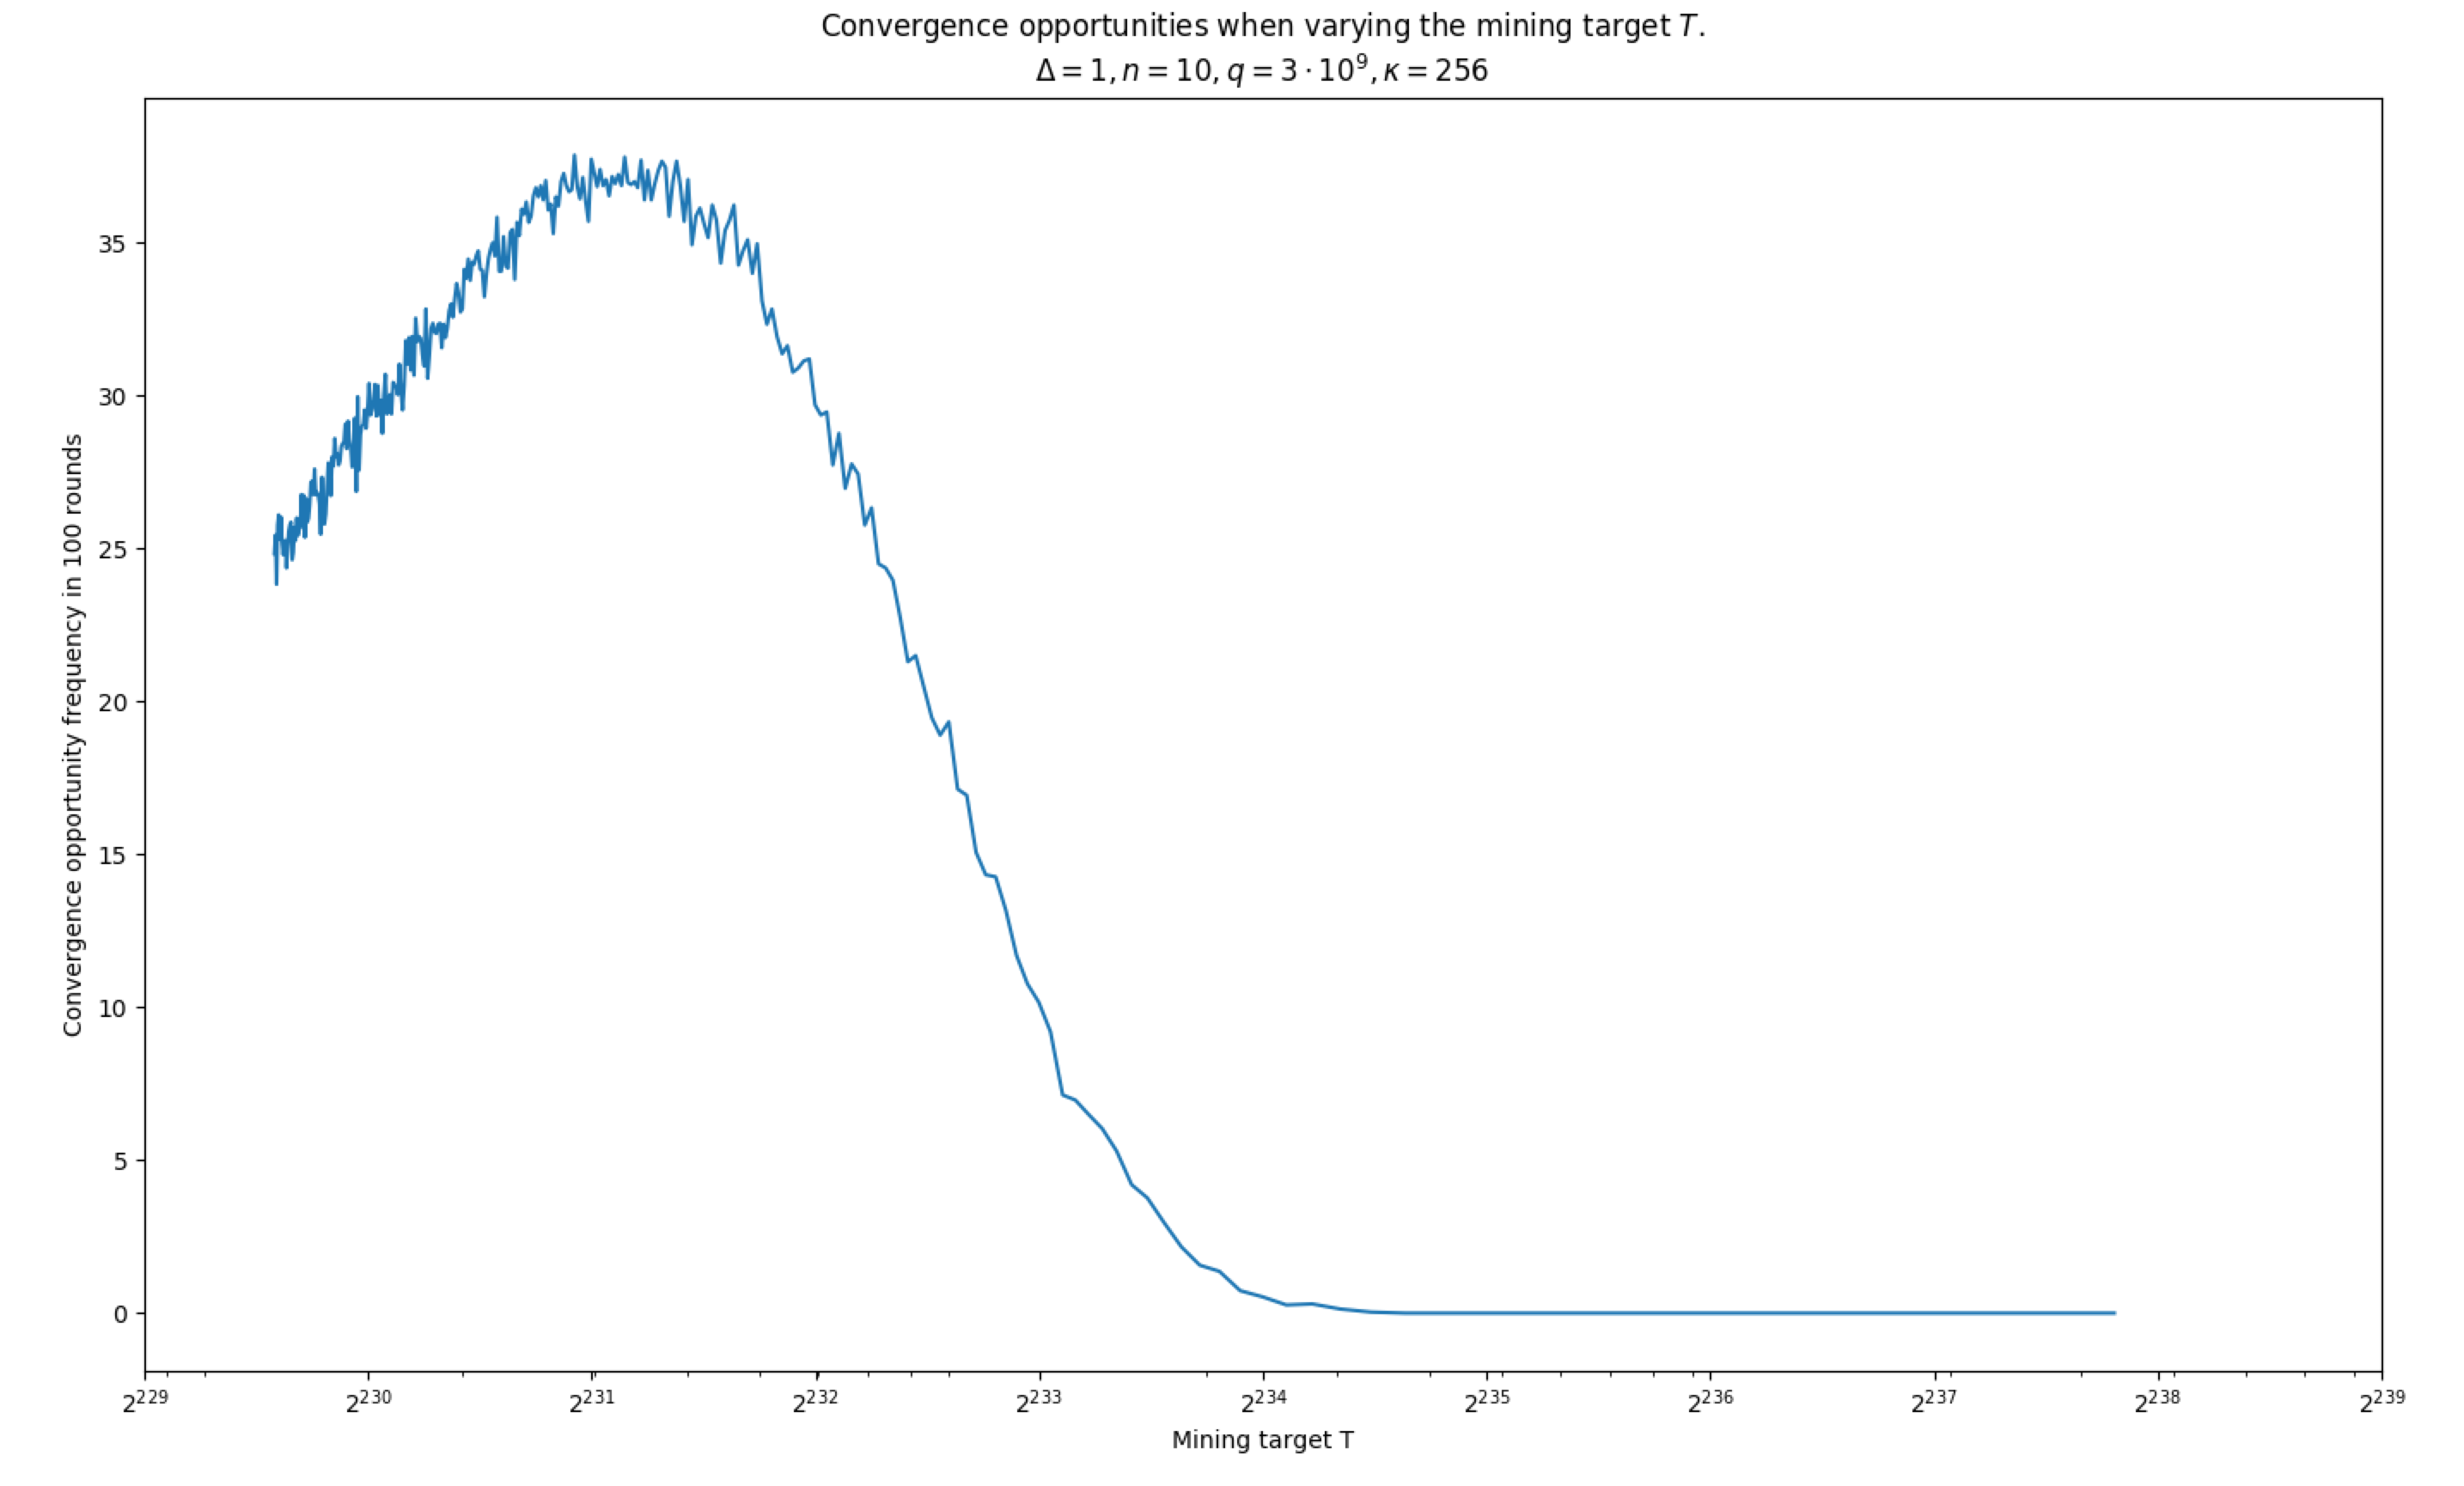
\includegraphics[scale=0.35]{figures/targetT.png}\]
%
% \label{fig:convergence_opp_frequency}
% \caption{Plot of convergence opportunity frequency versus target $T$}
% \end{figure}
\end{problems}

\section*{Further Reading}

The Nakamoto Race was explored in Satoshi's Bitcoin paper. There, he analyzed the probability of
the success of a minority adversary mounting the Nakamoto Race attack against a majority of honest
parties. This is the only attack that Satoshi analyzed. He did not prove that his protocol is secure
against all adversaries. The longest chain protocol was analyzed and proven secure against \emph{all}
adversaries in the later work of the Bitcoin Backbone, which we explore in the later chapters of this
book.

In an even later work from 2020,
\emph{Everything is a Race and Nakamoto Always Wins~\cite{nakamoto-wins}},
the authors discuss hod Satoshi has been right all along, but we did not know it:
In fact, \emph{any} mining attack an adversary can possibly perform is roughly equivalent
to a Nakamoto Race.

While the Fan-Out was known to Nakamoto, but was made precise in the Bitcoin Backbone line of
work, where they argue that

\begin{quote}
$f$ cannot be too large, because [this would mean] that uniquely
successful rounds will not produce sufficiently many PoW's to overcome the PoW's
produced by the adversary.
\end{quote}
